\chapter{Introduction}
\label{chap:intro}

\makeatletter
\newenvironment{chapquote}[2][2em]
{\setlength{\@tempdima}{#1} \def\chapquote@author{#2} \parshape 1
  \@tempdima \dimexpr\textwidth-2\@tempdima\relax \itshape}
{\par\normalfont\hfill--\
\chapquote@author\hspace*{\@tempdima}\par\bigskip}
\makeatother

\begin{chapquote}{Alan Turing}
  ``I propose to consider the question: Can machines think?''
\end{chapquote}
The ultimate goal of image understanding is to transfer visual
signals (images/videos) into abstract symbolic descriptions of the
world which are helpful for decision making.
However, understanding images is a not trivial task for machines.
In order to handle various complicated scenarios, researchers divide
image understanding into different computer vision tasks: pedestrian
detection for autonomous driving, face recognition for security
system, and image retrieval for image searching engines.

For many applications, knowing when, where, and in which direction a
picture was taken is important to understand the world. However, most
images does not carry such information, thus we need to develop
algorithms to dig them up.  We refer to the task of estimating these
properties as {\em geo-calibration}.
Most recent work of geo-calibration focus on deterministic systems, 
which have some drawbacks: 1) they can not model the inherent
uncertainties from images of ambiguous scenes, and 2) they can not be
used by applications that take probabilistic inputs. To address
these problems, we propose to build probabilistic models for camera
geo-calibration.

We also show that learning to geo-calibrate a camera is helpful for
high-level feature extracting. Feature engineering is essential for
image understanding. In recent years, learning based approaches for
high-level feature extracting like deep neural nets have drawn a lot
of attention due to the fact that they do not need any expert
knowledge about the target data. However, most of these feature
learning methods heavily relies on manually labeled data. In our
thesis, we presented alternative ways to learn high-level image
representations when the manually labeled data is either insufficient
or absent.

\begin{figure}
  \centering
  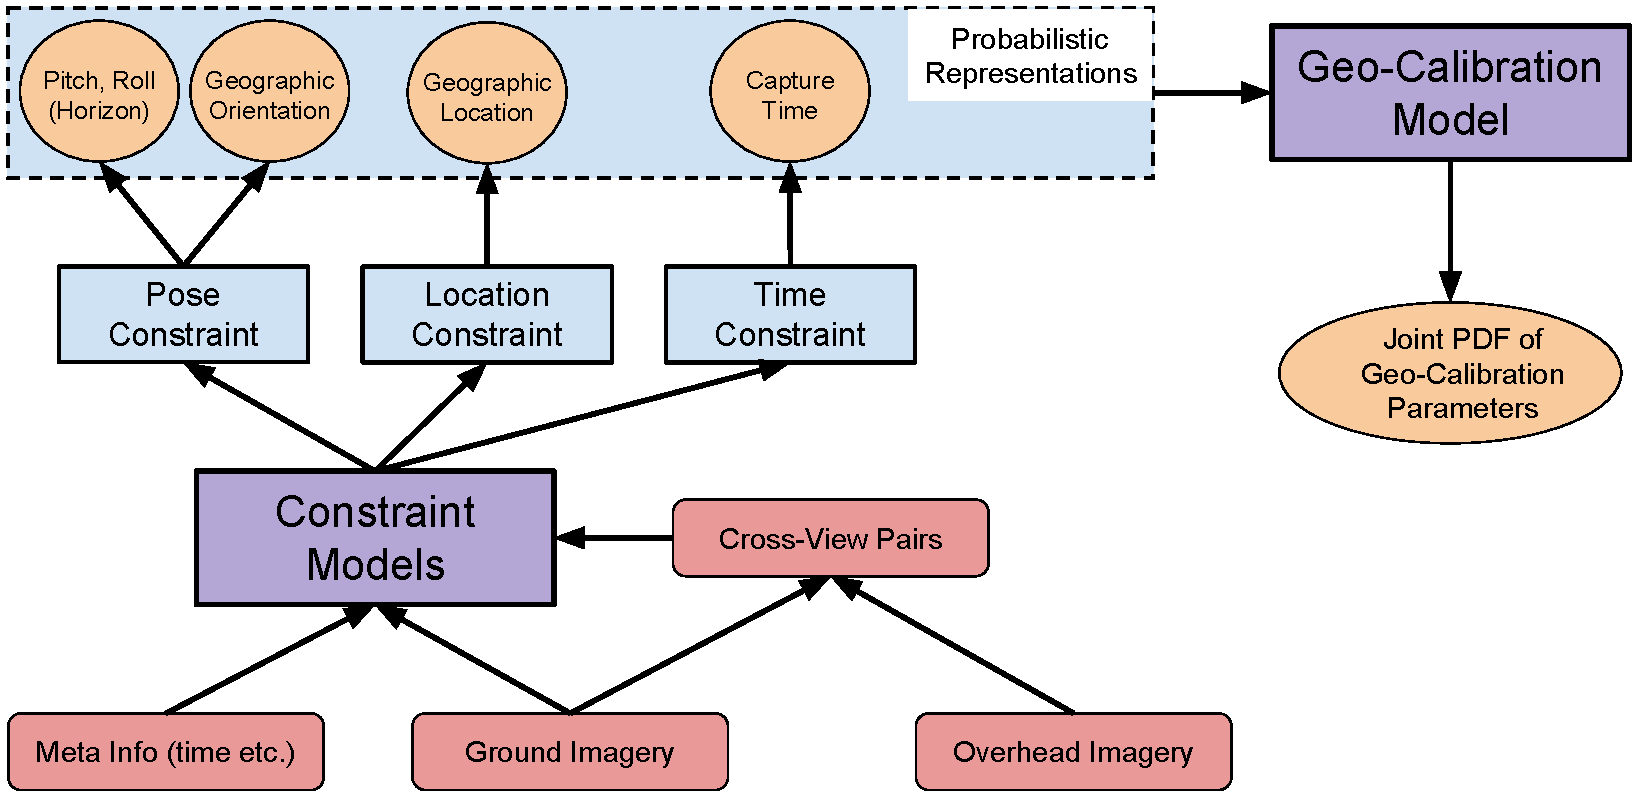
\includegraphics[width=.8\linewidth]{introduction/architecture}
  \caption{Architecture of our approach.}
  \label{fig:intro:architecture}
\end{figure}

\section{Background}

\subsection{Geo-Calibration}
%\todo{add deterministic methods}
%
Automatic image geo-calibration continues to grow in importance as a
direct result of the increasing amount of imagery available
via the Internet. Conceptually the geo-calibration task is
straightforward: given an image, identify the time and the location it
was captured in the world and the direction the camera was facing.
Solving this problem is of great value for a wide variety of fields,
with potential applications ranging from the forensic
sciences~\cite{stylianou13jane} to environmental
monitoring~\cite{zhang2012mining}.
\todo{make it smoother}

\begin{itemize}[noitemsep]
\item \textbf{Geo-Localization:}
Extracting location-dependent or orientation-dependent features from
image data has drawn a great detail of attention from the vision
community~\cite{jacobs07geolocate, jacobs11geolocate,
jacobs08geoorient}. The common trend amongst these methods is that
they take advantage of a large dataset of geo-referenced images. Hays
and Efros~\cite{hays2008im2gps} use a data-driven scene matching
approach to localize a query image using a large dataset of geo-tagged
images.  Doersch \etal~\cite{doersch2012what} extract
location-dependent features that capture the relative appearance
differences of large cities.  Lin et al.~\cite{lin2013cross} localize
a ground-level image by learning the relationship between pairs of
ground and aerial images of the same location. Other techniques focus
on urban environments and infer location using local image
descriptors~\cite{schindler2008detecting,snavely2006photo}. Li et
al.~\cite{li2012worldwide} exploit geo-registered 3D points clouds to
estimate camera pose. Many other cues exist, such as the
skyline~\cite{baatz2012large,ramalingam2009geolocalization}, sky
appearance~\cite{lalonde2010sun,workman2014rainbow}, and
shadows~\cite{junejo2008estimating,wu2010geo}.
\newline

\item \textbf{Time Estimation:}
Matzen and Snavely~\cite{matzen2014scene} predict
timestamps for photos by matching against a time-varying
reconstruction of a scene.  Hill~\cite{hill1994elephant} estimate the
time of the day by measuring the light intensity profiles captured by
cameras. Methods are proposed to date the
year book photos by analyzing human
appearance~\cite{salem2016face2year,ginosar2015century}. Lee
\etal~\cite{linking2015iccp} find visual paterns in the buildings,
relate them to certain time periods.
\newline

\item \textbf{Camera Pose Estimation:}
\todo{}

\end{itemize}

\subsection{Deep Learning in Geo-Calibration}
In recent years, deep neural networks (DNNs) were proven to be
extremely successful in many computer vision areas. 
It is widely accepted that DNNs have excellent performance in
high-level visual feature learning.
This valuable ability provides researchers powerful tools to
solve the challenging geo-calibration tasks.
Weyand and Kostrikov \etal~\cite{planet} propose a convolutional
network to predict the geographic location of the input
image. Walch \etal~\cite{walch2017image} aggregate learned CNN
features with LSTM to generate global image representation for camera
localization.  In pose estimation aera, Work~\cite{zhai2016horizon,
workman2016horizon, hold2017perceptual} has been done to to identify
the horizon line with CNNs (one can derive the camera roll and pitch
angles from the horizon line position giving the camera focal length).

Closely related to camera geo-calibration, studies also have been done
to identify the camera intrinsics using deep neural networks.
Workman \etal~\cite{workman2015deepfocal} develop a CNN to estimate the camera
focal length. Kendall \etal~\cite{kendall2015convolutional} propose a
neural network that can identify 6-DOF camera parameters, but their
method only limited to specific scenes.


\subsection{Ground-to-Aerial Geo-Calibration}
Data-driven scene matching approaches are widely used to localize a
query image by registering in a large dataset of geo-tagged
images~\cite{im2gps, li2010location,zamir2010accurate}.
Benefited from the fast growing monitoring satellite and drone markets,
geo-tagged satellite/aerial imagery becomes more and more available
than ever before, which makes it a rich source for building
reference database. We refer to the geo-calibration methods which use
the aerial imagery as geographic reference as {\em Ground-to-Aerial
Geo-Calibration}.

Cross-view image pair is the basic element for ground-to-aerial
geo-calibration. It consists of a ground-level image and an overhead
image at the same location. In some cases, two images may also be aligned
in orientation. 

Recent work on ground-to-aerial
geo-localization~\cite{lin2013cross,lin2015learning,workman2015geocnn,workman2015wide}
has shown that convolutional neural networks are capable of extracting
features from geo-tagged aerial imagery that can be matched to features extracted
from the inquiry ground imagery.  Vo \etal~\cite{vo2016localizing} extend this
line of work, demonstrating improved geo-localization performance by
applying an auxiliary loss function to regress the ground-level camera
orientation with respect to the aerial image. Hu and Feng
\etal~\cite{mh2018cvm} achieve the state-of-the-art performance in
geo-localization by extracting cross-domain global features using
the NetVLAD~\cite{arandjelovic2016netvlad} technique.


\subsection{Geo-Calibration for Feature Learning}

Automatic feature engineering has drawn a lot of attention over the
past years in the computer vision community due to its efficiency and
not requiring expert knowledge about the data. Deep neural networks
are wildly accepted by researchers as good tools to learn high-level
image representations.
The most commonly used approach for deep feature learning is
full supervision, which usually requires manually annotated
data~\cite{yosinski2014transferable,zhou2016learning,wen2016discriminative}.
Though full supervision work well in many applications, there are
exponentially more image resources without manual annotation (cell
phone imagery, YouTube videos\etc), which show a huge potential for
visual feature learning.   

To exploit these unlabeled data, recent work has explored the use of
self-supervision (sometimes referred to as unsupervised learning or
pretext tasks) for training deep neural networks that capture useful
visual representations~\cite{doersch2015unsupervised,pathak2016context}. 
These methods typically
exploit some known quantity of the data (e.g., pixel color values) to
avoid expensive manual annotation. As a byproduct, a useful visual
representation is learned.
For example, Zhang et al.~\cite{zhang2016colorful} show how image
colorization (synthesizing colors for a grayscale image) is a powerful
pretext task for learning visual representations. Pathak et
al.~\cite{pathak2017learning} exploit low-level motion-based grouping
cues for unsupervised feature learning.  
%
As new learning technique address the lack of massive amounts of
labeled data, domain adaptation adapt the feature generating model to
another feature domain so that it improve the performance when dealing
with new input
data~\cite{fernando2013unsupervised,fernando2015joint,saenko2010adapting,wang2016actions,tinghui2016flow}.
Duan \etal~\cite{duan2012learning} proposed to learn a linear
projection to transfer from the source feature subspace to the target
subspace. Sohn \etal~\cite{sohn2017unsupervised} improved the
performance of video face recognition using an adversarial-based
approach to adapt the network to unlabled video imagery.

%\section{\todo{Dataset}}
%Introduce the dataset we use.

\section{Our Approach}
Our approach consists of two big steps. First, we propose a general
probabilistic model to jointly estimate the geo-calibration
parameters. The key for the success of this model is to construct good
constraint functions which describe the fitness between the calibration
parameters and the images. As the second step of our approach, we
dismantle the full geo-calibration into several partial
geo-calibration tasks, each of which could provides a strong constraint
function that fits in the general model. The architecture of
our approaches refers to \figref{intro:architecture}.
%
In the end, we show that learning to geo-calibrate a camera is helpful
for high-level image feature extracting.


\subsection{General Probabilistic Model for Geo-Calibration}
The complete camera geo-calibration detects the camera
geographic location, pose, and focal length of the camera.  We
design a general model to estimate the probability over these
geo-calibration parameters: First, we model the relationship between the
image projection of the scene and the geo-calibration parameters. This
relationship can be described by the pin-hole model, and
the geographic location of the camera.
We then construct a scoring function to measure the ``fitness'' between the
calibration parameters and the observation of the image. 
The scoring function is proportional to the probability distribution
of the camera parameters. We propose a Markov Chain Monte
Carlo (MCMC) sampling approach to approximate the underlying
probability distribution over the full geo-calibration of the camera.
Our model is a general architecture, which can take different
constraints to form the scoring function. The details about this model
can be found in \chapref{mcmc}.

\subsection{Developing Constraint Functions}
In our general model, the scoring function is defined as a linear
combination of multiple constraint functions.
In the rest of the work, we focus on developing good constraint
functions for different set of calibration parameters. 

\begin{itemize}[noitemsep]
  \item \textbf{Constraint for Horizon Line and Vanishing Points:}
  We first estimate camera roll and pitch angles. Assuming the intrinsic
  parameters are known, camera roll and pitch angles can be
  derived from the horizon line position in the image. Compared to
  directly detecting the camera pose, identifying horizon line is easier
  because it is tightly related to the appearance
  of the scene. In our work, we create a new method using CNN to
  estimate the prior distribution of the horizon line. We assign
  a probability to each horizon line by measuring their consistences
  with vanishing points detected using traditional statistic methods.
  We present the algorithm details in \chapref{fasthorizon}.
  \newline

  \item \textbf{Constraint for Time and Coarse Geographic Locations:}
  In this work, we demonstrate to estimate the capture time and the
  camera geographic location given the input image.
  Our network has two heads to predict the image
  capture time and the geographic location jointly.
  For time estimation, our network is able to predict the
  joint distribution over the month of the year and the global hour of the
  day when the input image has been captured.
  For camera geo-localization, We provide two approaches to obtain the
  probability distribution over the camera geographic location. Most
  straightforwardly, our network estimate the categorical distribution
  over location of the world, which is represented as a $N \times M$
  meshgrid. Better results can be procured with image capture time as
  auxiliary input (if it is known). 
  %Our algorithm can also compute the probability at arbitrary
  %geographic location, with lower accuracy than the straightforward
  %method.
  We will present the algorithm details in \chapref{whenwhere}.
  \newline

  \item \textbf{Constraint for Fine Geographic Locations and Orientations:}
  In our previous method, we present that our algorithm can estimate
  the camera location distribution in low-res world division. In this
  work we focus on refining the geo-localization results with the help
  of overhead imagery and on estimating geo-orientation of the camera. 
  We first learn to segment the ground scene from its paired aerial image.
  When refining the camera geographic location, we compare the
  semantic layout of the ground image with the semantic layout
  transferred from overhead images, which are sampled in different
  locations and orientation angles. The optimal prediction is found when the
  semantic layouts from these two sources match best. For probabilistic
  outputs, we assign a score to each location and orientation setting,
  based on how well the semantic layouts match to each other. We will
  present the algorithm details in \chapref{crosstransf}.
  \newline

\end{itemize}


\subsection{Geo-Calibration for Feature Learning}
Our methods also focus on lavaging the camera geographic information to
deal with the challenges of lacking manually annotated data during DNN
training. The insight is that the camera geographic information
encodes semantic information because it is related to the
appearances of the scenes.

\begin{itemize}[noitemsep]
  \item \textbf{Ground-to-Aerial Feature Learning:}
  Current machine learning methods address problems that involves mostly
  the ground-level imagery. Tons of dataset targeting on ground imagery are
  annotated while much fewer are done for the satellite/aerial imagery. In
  \chapref{crosstransf}, we proposed a method to learn the aerial image
  semantic segmentation with only ground-level ground truth. Our method
  exploits the spatial correspondences between images in cross-view
  pairs. 
  In this work, we try to transfer the semantics from the ground
  imagery to the aerial imagery by identifying the latent geometry
  correspondences between these two. Similar to the monocular depth
  estimation methods that driven by the technique called {\em
  Reprojection Losses}~\cite{garg2016unsupervised,
  godard2017unsupervised,zhou2017unsupervised, yan2016perspective}, our
  network learns to geometrically project pixels from the aerial
  images to the ground images, and to segment the aerial images
  jointly.
  \newline

  \item \textbf{Geo-Temporal Feature Learning:}
  In \chapref{whenwhere}, we demonstrate that our algorithm is able to
  learn geo-temporal image representations with geographic locations and
  capture time.
  Our work is most similar to Li and Snavely~\cite{li2018learning},
  who propose an approach for learning intrinsic images by observing
  image sequences with varying illumination over time. While their
  targets are reflectance and shading images of the scene, we consider
  two novel pretext tasks, time and location estimation.
  By learning to predict the geographic location and capture time of
  the query image, our network learns to extract geo-temporal features
  from the image.

\end{itemize}
